\documentclass[12pt, twoside]{article}
\usepackage{fancyhdr, setspace, tikz}
\usepackage[margin = 1.0in]{geometry}
\usepackage[format=plain, labelfont={bf,it}, textfont=it]{caption}
\usepackage{hyperref}
\setstretch{1.15}			% Line spacing

\pagestyle{fancy}
\raggedbottom
\usepackage[bottom]{footmisc}
\setlength{\parindent}{0cm}
\setlength{\parskip}{0.5\baselineskip}

\usetikzlibrary{positioning,shapes.geometric}
\newcommand{\Rx}{
	\kern0.71mm
	\makebox[0pt][c]{
	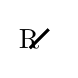
\begin{tikzpicture}[baseline]
		\node [anchor=base, inner sep=0pt] at (0,0) {\makebox[0pt][c]{R}};
		\draw [line width=0.4mm] (0.01,0) -- (0.25,0.24);
	\end{tikzpicture}
	}
	\kern-0.72mm
}\newcommand{\rx}{
	\kern0.71mm
	\makebox[0pt][c]{
	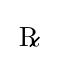
\begin{tikzpicture}[baseline]
		\node [anchor=base, inner sep=0pt] at (0,0) {\makebox[0pt][c]{R}};
		\draw [line width=0.2mm] (0.01,0) -- (0.13,0.12);
	\end{tikzpicture}
	}
	\kern-0.52mm
}

\newcommand{\name}{Raleigh Ems and Dan Kats}
\newcommand{\myTitle}{\Rx evolving Door}
\newcommand{\mytitle}{\rx evolving Door}

\begin{document}
	
	\fancyhead[EOL]{\textsc{\mytitle}}
	\fancyhead[EOR]{\name}

	\pagenumbering{alph}
	\begin{titlepage}
		\vspace*{\fill}

		\begin{center}
			{\Huge \myTitle \\[1.5cm]}
			{\LARGE \name \\}
			{\large \href{mailto:rde17@case.edu}{rde17@case.edu} $|$ \href{mailto:djk175@case.edu}{djk175@case.edu} \\[0.5cm]}
		\end{center}

		\vspace*{\fill}
	\end{titlepage}
	\pagenumbering{arabic}
	
	There are not many interactive options for medical school studying, aside from quizzing each other. We want to change this by creating an infinitely expandable role-playing game that will put medical students into virtual clinical situations. Students will manage patients that are generated from a set of parameters, so no case will appear more than once in the same presentation. The player will have to work up the patients, give a diagnosis, and pick a treatment plan, just like they are expected to do for the rest of their lives.

	The screen will start as a bunch of beds, which will gradually fill and empty as patients are admitted and treated (Figure~\ref{fig:home}).

	\begin{figure}[h]
		\centering
		\includegraphics[width=0.8\textwidth]{../Figures/Home/Home.pdf}
		\caption{A sample home screen to view all current patients.}
		\label{fig:home}
	\end{figure}

	To manage each patient, clicking on them will open a chart-like screen (Figure~\ref{fig:chartmain}). Each patient will start out with some basic information, but not all of the information necessary for diagnosis will be given. Through the ``Orders'' tab, the player will be able to ask the patient more questions, perform physical exam maneuvers, and order labs and imaging. In the ``Treatment'' tab, the player can establish a diagnosis and select the proper treatment. Once this is done, the patient encounter will end and a summary will appear, describing what the patient's actual diagnosis was, the proper/necessary physical exam findings, labs, and imaging needed for diagnosis, and the proper treatment plan.

	\begin{figure}[h]
		\centering
		\includegraphics[width=0.8\textwidth]{../Figures/ChartMain/ChartMain.pdf}
		\caption{The History of Present Illness page of a sample patient's chart.}
		\label{fig:chartmain}
	\end{figure}

	Rather than having one patient present at a time, we intend to have several patients circulating through a room of beds. Each ``Order'' action that the player takes will come with a time cost that will impact all patients (e.g.\ performing 5 maneuvers in order to assess an acute abdomen will take some time, say 10 minutes; taking a thorough travel history will also take some amount of time, say 20 minutes). Rather than having some abstract life points, each patient will have a certain time left in their lives (specific to their pathology). As a result, performing unnecessary histories and physicals will lead to \emph{all} patients losing time, making it necessary for the player to pick and choose what is necessary, as well as prioritizing some patients over others. The red bars in Figure~\ref{fig:home} are a representation of how much time each patient has left, and can be toggled on/off to make gameplay easier/harder.

	The ``Notes'' tab (Figure~\ref{fig:chartmain}) is a free-text field for the player to make notes with (e.g.\ a working differential diagnosis, plan, etc.).

	The key of this game is that no two patients will be the same. With help from faculty (hopefully, \emph{you}), we will compile a database of various parameters for each disease. This will consist of many variables, such as age range, common signs and symptoms, occassional signs and symptoms, common physical exam findings, occassional physical exam findings, etc.). The game will create new presentations of each disease based on these parameters, also adding extra information (e.g.\ non-specific history and physical exam findings, past medical history, family medical history, social history, etc.) that will serve to keep each presentation from being the ``classical case''.

	To add some more fun, we will also have an attending walking around the screen, ``pimping'' the player at random intervals with questions (e.g.\ basic science, pathophysiology) that would not otherwise appear.

	\vspace*{\fill}
	\begin{center}
		\Large
		Please help us build our database! {\color{blue}\underline{\href{https://goo.gl/forms/FWQe1oZEc9khfdRl1}{Click here to go to our online submission form.}}}

		\vspace{24pt}
		Help us get the word out by sharing with your colleagues.

		Thank you!
	\end{center}
	\vspace*{\fill}

\end{document}